\begin{prob}
    \begin{subprobset}
        \begin{subprob}
	        Run Dijkstra's Algorithm on the following graph using node $a$ as the source.  Below each node $u$, write the shortest path length from $a$ to $u$.  Mark the predecessor of $u$ by highlighting it or making a bold arrow.  
            \begin{center}
                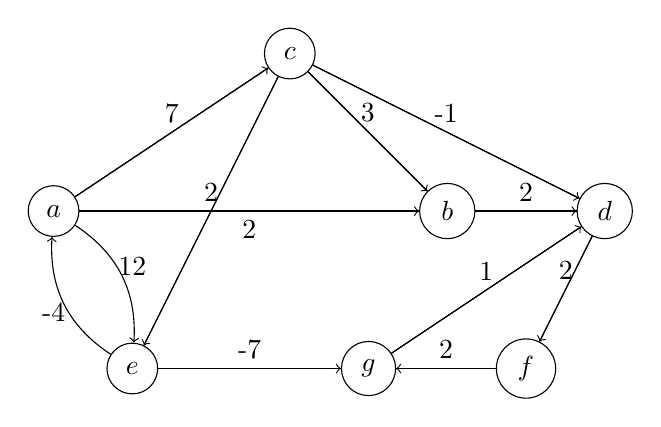
\begin{tikzpicture}
                    \tikzset{
                        vertex/.style={draw, circle, text width=8, align=center},arc/.style={->}
                    }
                    
                    \draw node[vertex] (a) at (0,0) {$a$};
                    \draw node[vertex] (b) at (5,0) {$b$};
                    \draw node[vertex] (c) at (3,2) {$c$};
                    \draw node[vertex] (d) at (7,0) {$d$};
                    \draw node[vertex] (e) at (1,-2) {$e$};
                    \draw node[vertex] (f) at (6,-2) {$f$};		
                    \draw node[vertex] (g) at (4,-2) {$g$};		
                    \foreach \x/\y in {%
                        a/b, a/c,b/d,c/e,c/b,c/d,d/f,f/g,e/g,g/d%
                    }{
                    \draw (\x) edge[arc] (\y);
                    }
                    \draw (a) edge[arc, bend left] (e);
                    \draw (e) edge[arc, bend left] (a);
                    \draw[-] (a) -- node[below] {2} (b);
                    \draw[-] (a) -- node[above] {7} (c);
                    \draw (a)   node[below=30pt] {-4} (e);
                    \draw (e)   node[above=30pt] {12} (a);
                    \draw[-] (b) -- node[above] {2} (d);
                    \draw[-] (c) -- node[above] {3} (b);
                    \draw[-] (c) -- node[above] {2} (e);
                    \draw[-] (c) -- node[above] {-1} (d);
                    \draw[-] (d) -- node[above] {2} (f);
                    \draw[-] (e) -- node[above] {-7} (g);
                    \draw[-] (f) -- node[above] {2} (g);
                    \draw[-] (g) -- node[above] {1} (d);
                \end{tikzpicture}
            \end{center}
	
            \begin{soln}
                \begin{center}
                    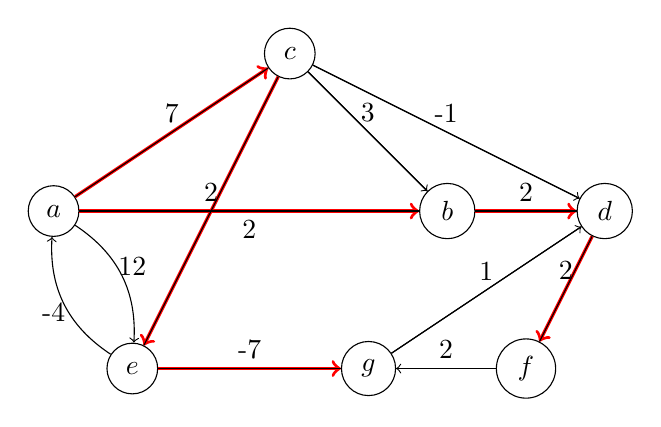
\begin{tikzpicture}
                    \tikzset{
                        vertex/.style={draw, circle, text width=8, align=center},arc/.style={->}
                    }
                    
                    \draw node[vertex] (a) at (0,0) {$a$};
                    \draw node[vertex] (b) at (5,0) {$b$};
                    \draw node[vertex] (c) at (3,2) {$c$};
                    \draw node[vertex] (d) at (7,0) {$d$};
                    \draw node[vertex] (e) at (1,-2) {$e$};
                    \draw node[vertex] (f) at (6,-2) {$f$};		
                    \draw node[vertex] (g) at (4,-2) {$g$};		
                    \foreach \x/\y in {%
                        c/b,c/d,f/g,g/d%
                    }{
                    \draw (\x) edge[arc] (\y);
                    }
                    \foreach \x/\y in {%
                        a/b, a/c,b/d,c/e,d/f,e/g%
                    }{
                    \draw (\x) edge[very thick, red, ->] (\y);
                    }
                    \draw (a) edge[arc, bend left] (e);
                    \draw (e) edge[arc, bend left] (a);
                    \draw[-] (a) -- node[below] {2} (b);
                    \draw[-] (a) -- node[above] {7} (c);
                    \draw (a)   node[below=30pt] {-4} (e);
                    \draw (e)   node[above=30pt] {12} (a);
                    \draw[-] (b) -- node[above] {2} (d);
                    \draw[-] (c) -- node[above] {3} (b);
                    \draw[-] (c) -- node[above] {2} (e);
                    \draw[-] (c) -- node[above] {-1} (d);
                    \draw[-] (d) -- node[above] {2} (f);
                    \draw[-] (e) -- node[above] {-7} (g);
                    \draw[-] (f) -- node[above] {2} (g);
                    \draw[-] (g) -- node[above] {1} (d);
                    \end{tikzpicture}
                \end{center}
                est = \{
                'a': 0,
                'b': 2,
                'c': 7,
                'd': 4.
                'e': 9,
                'f': 6,
                'g': 2
                \}
            \end{soln}
        \end{subprob}
    
        \begin{subprob}
        	Dijkstra’s algorithm found the wrong path to some of the vertices. 
        	For just the vertices wherethe wrong path was computed, indicate both the path that was computed and the correct path.
        	\begin{soln}
                \\
                Computed path to d is a,b,d but shortest path is a,c,e,g,d.
                \\
                Computed path to f is a,b,d,f but shortest path is a,c,e,g,d,f.
            \end{soln}
            \vspace{3em}
        \end{subprob}
        \begin{subprob}
        	What single edge could be removed from the graph such that Dijkstra’s algorithm would happen to compute correct answers for all vertices in the remaining graph?
        	\begin{soln}
                (e,g)
            \end{soln}
            \vspace{2em}
        \end{subprob}
    \end{subprobset}
\end{prob}
